% ------------------------------------------------------------------------------
% TYPO3 Version 9.1 - What's New - Chapter "Changes for Integrators" (Italian Version)
%
% @author	Michael Schams <schams.net>
% @license	Creative Commons BY-NC-SA 3.0
% @link		http://typo3.org/download/release-notes/whats-new/
% @language	English
% ------------------------------------------------------------------------------
% LTXE-CHAPTER-UID:		3a9852ea-e2360d9d-1ff5eec1-a7de3f9f
% LTXE-CHAPTER-NAME:	Changes for Integrators
% ------------------------------------------------------------------------------

\section{Modifiche per integratori}
\begin{frame}[fragile]
	\frametitle{Modifiche per integratori}

	\begin{center}\huge{Capitolo 2:}\end{center}
	\begin{center}\huge{\color{typo3darkgrey}\textbf{Modifiche per integratori}}\end{center}

\end{frame}

% ------------------------------------------------------------------------------
% LTXE-SLIDE-START
% LTXE-SLIDE-UID:		91278b9f-e2a8b1d4-f724bfa7-1337855d
% LTXE-SLIDE-ORIGIN:	31b70474-edcc2a8a-d4a5fd3d-58734dc5 English
% LTXE-SLIDE-TITLE:		EXT:impexp - Maximum Number Of Records Restriction Removed
% LTXE-SLIDE-REFERENCE:	Deprecation-83592-ImpexpRemovedMaximumNumberOfRecordsRestriction
% ------------------------------------------------------------------------------

\begin{frame}[fragile]
	\frametitle{Modifiche per integratori}
	\framesubtitle{Import/Export}

	Sono stati apportati diversi aggiornamenti alla estensione di sistema \texttt{impexp}:

	\begin{itemize}
		\item La restrizione "numero massimo di record" è stata rimossa\newline
			\smaller
				Quando si esportano pagine o record, la restrizione di esportazione
				solo un numero massimo di record, è stata rimossa.
			\normalsize

		\item La restrizione "dimensione massima dei file" è stata rimossa\newline
			\smaller
				Quando si esportano file usando l'interfaccia "Export", la
				restrizione esporta solo file fino ad una dimensione massima,
				è stata rimossa.
			\normalsize

		\item Rimossa verifica dimensione dei file \newline
			\smaller
				Quando si esportano o importano strutture, record e file veniva archiviata
				la dimensione dei file esportati e verificata nel processo di importazione.
				Questo cambiamento non ha impatti sugli editori.
			\normalsize

	\end{itemize}

\end{frame}

% ------------------------------------------------------------------------------
% LTXE-SLIDE-START
% LTXE-SLIDE-UID:		66cb4148-198c6f16-4b395fc4-7296fe6b
% LTXE-SLIDE-ORIGIN:	0504ca33-7c23eff4-93a728fa-bd911c92 English
% LTXE-SLIDE-TITLE:		Redirect Functionality Moved To Redirects Module
% LTXE-SLIDE-REFERENCE:	83638-RedirectFunctionalityMovedFromSys_domainToRedirectsModule
% ------------------------------------------------------------------------------

\begin{frame}[fragile]
	\frametitle{Modifiche per integratori}
	\framesubtitle{Funzionalità di reindirizzamento}

	\begin{itemize}
		\item L'opzione per configurare un reindirizzamento, quando un dominio è aggiunto ad una specifica
			pagina o ramo di pagine, è stato rimossa.
		\item Le impostazioni di redirect possono ora essere fatte nel nuovo modulo\newline
			\textbf{Site Management} \textrightarrow \textbf{Redirects}
	\end{itemize}

	\begin{figure}
		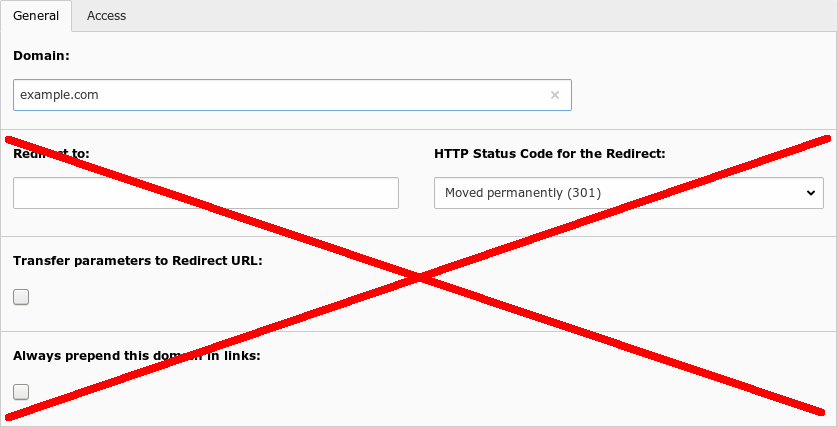
\includegraphics[width=0.6\linewidth]{ChangesForIntegrators/RedirectFunctionalityMovedToRedirectsModule.png}
	\end{figure}

\end{frame}

% ------------------------------------------------------------------------------
